%%%%%%%%%%%%%%%%%%%%%%%%%%%%%%%%%%%%%%%%%%%%%%%%%%%%%%%%%%%
% EPFL report package, main thesis file
% Goal: provide formatting for theses and project reports
% Author: Mathias Payer <mathias.payer@epfl.ch>
%
% This work may be distributed and/or modified under the
% conditions of the LaTeX Project Public License, either version 1.3
% of this license or (at your option) any later version.
% The latest version of this license is in
%   http://www.latex-project.org/lppl.txt
%
%%%%%%%%%%%%%%%%%%%%%%%%%%%%%%%%%%%%%%%%%%%%%%%%%%%%%%%%%%%
\documentclass[a4paper,11pt,oneside]{report}
% Options: MScThesis, BScThesis, MScProject, BScProject
\usepackage[MScThesis,lablogo]{EPFLreport}
\usepackage{datetime}
\usepackage{amsmath}
\usepackage{amssymb}
\usepackage{xspace}
\usepackage{array}
\usepackage{lscape}
\usepackage{booktabs}
\usepackage{subcaption}
\usepackage{gensymb}
\usepackage{stmaryrd}


\usepackage{hyperref}
\usepackage{graphicx}

\title{Regional Climate Model Emulator based on Deep Learning: future SMB predictions over Antarctica}
\author{Marijn van der Meer}
\supervisor{Sophie de Roda Husman}
\adviser{Prof. Dr. sc. EPFL Martin Jäggi}
\expert{Prof. Dr. sc. TU Delft Stef Lhermitte}

\newcommand{\sysname}{FooSystem\xspace}

\begin{document}
\maketitle
\makededication
\makeacks

\begin{abstract}
The \sysname tool enables lateral decomposition of a multi-dimensional
flux compensator along the timing and space axes.

The abstract serves as an executive summary of your project.
Your abstract should cover at least the following topics, 1-2 sentences for
each: what area you are in, the problem you focus on, why existing work is
insufficient, what the high-level intuition of your work is, maybe a neat
design or implementation decision, and key results of your evaluation.
\end{abstract}

\begin{frenchabstract}
For a doctoral thesis, you have to provide a French translation of the
English abstract. For other projects this is optional.
\end{frenchabstract}

\maketoc

%%%%%%%%%%%%%%%%%%%%%%
\chapter{Introduction}
%%%%%%%%%%%%%%%%%%%%%%

The introduction is a longer writeup that gently eases the reader into your
thesis~\cite{dinesh20oakland}. Use the first paragraph to discuss the setting.
In the second paragraph you can introduce the main challenge that you see.
The third paragraph lists why related work is insufficient.
The fourth and fifth paragraphs discuss your approach and why it is needed.
The sixth paragraph will introduce your thesis statement. Think how you can
distill the essence of your thesis into a single sentence.
The seventh paragraph will highlight some of your results
The eights paragraph discusses your core contribution.

This section is usually 3-5 pages.

%%%%%%%%%%%%%%%%%%%%
\chapter{State of the art}
%%%%%%%%%%%%%%%%%%%%

The related work section covers closely related work. Here you can highlight
the related work, how it solved the problem, and why it solved a different
problem. Do not play down the importance of related work, all of these
systems have been published and evaluated! Say what is different and how
you overcome some of the weaknesses of related work by discussing the 
trade-offs. Stay positive!

This section is usually 3-5 pages.

\section{Regional Climate Model Emulator based on Deep Learning: Concept and First Evaluation of a Novel Hybrid Downscaling Approach \cite{Doury}}
This paper proposes a novel hybrid downscaling approach that emulates the downscaling function of a a regional climate model.

\begin{itemize}
\item RCM: EURO-CORDEX simulations based on the CNRM-ALADIN63, 1951-2100 RCP4.5 and RCP8.5
\item GCM: CNRM-CM5 used in CMIP5 → 6h frequency + sea surface temperature, sea ice cover and aerosol optical depth at monthly frequency
\item ML model learns the RCM transformation of the large-scale climate information into local-scale
\item Target variable: near surface temperature (TAS)
\item Target domain: southwest European domain
\item Historical period: 1951 to 2005
\item Scenarios (2006-2100): based on two Representative Concentration Pathways from CMIP5; RCP4.5 and RCP8.5
\end{itemize}
Computational performance:
\begin{itemize}
    \item U-Net: fully convolutional neural network algorithm
    \item Substantial computational gain regarding RCM computational cost
    \begin{itemize}
        \item 2h training on GPU + downscaling instantaneous
        \item RCM simulation involves weeks of computation on super-computer
    \end{itemize}
\end{itemize}
Training of model 
\begin{itemize}
    \item RCM can be broken down into a large scale transformation and a downscaling function
    \item Training using existing RCM simulations → learn large scale/local scale relationship in different climates and in future climate
    \item Training in perfect model framework: input and output to ML model come from same RCM simulation → focus on downscaling function
    \item Input variable: daily large-scale and low-resolution RCM information (upsampled to GCM like resolution)
    \item Output variable: daily maps of TAS at RCM resolution (~12km)
    \item Emulator is RCM-dependent as downscaling function depends on RCM choice
\end{itemize}
Results
\begin{itemize}
    \item Emulator evaluated in both perfect model (evaluation 1) and GCM worlds (evaluation 2)
    \item capture very well transformation from low resolution information to high resolution TAS
    \item robust to different sources of input
    \item succeeds very well in reproducing high resolution spatial structure and daily variability of the RCM
    \item evaluation 1 shows that emulator is able to reproduce original series almost perfectly
    \item training emulator in future climate improves its ability to reproduce warmer climate
    \item limitations in accurately simulating extreme events and complete climate change magnitude
    \item RCM-GCM large scales inconsistencies when evaluating on GCM. Does not learn to reproduce large scale transformations (because trained only on RCM)
\end{itemize}
\section{Diverging future surface mass balance between the Antarctic ice shelves and grounded ice sheet \cite{Kittel}}

\section{SmaAt-UNet: Precipitation Nowcasting using a Small Attention-UNet Architecture~\cite{smatunet}}


%%%%%%%%%%%%%%%%
\chapter{Model and methods}
%%%%%%%%%%%%%%%%

\begin{table}[!tbp]
    \centering
    \caption{}
    \renewcommand\arraystretch{1.5}
    \begin{tabular}{l>{\raggedright\arraybackslash}p{0.4\linewidth}>{\raggedright\arraybackslash}p{0.4\linewidth}}
    \toprule
        \textbf{Notation} & \textbf{Description} & \textbf{Dimensions} \\ \toprule 
        $\mathcal{D}$ & Input Domain & $\llbracket 1, I \rrbracket \times \llbracket 1, J \rrbracket$   \\
        $\mathcal{E}$ & Target Domain & $\llbracket 1, K \rrbracket \times \llbracket 1, L \rrbracket$   \\
        $(i,j)$ & Spatial indexes over
        input grid & $\mathcal{D}$   \\
        $(k,l)$ & Spatial indexes over
        target grid & $\mathcal{E}$   \\
        $X$ & Input: set of 2D variables over $\mathcal{D}$ & $T \times \llbracket 1, I \rrbracket \times \llbracket 1, J \rrbracket \times C_1$   \\
        $Z$ & Input: set of 1D variables over $\mathcal{D}$ & $T \times C_2$   \\
        $Y$ & Target: surface mass balance over $\mathcal{E}$ & $T \times \llbracket 1, K \rrbracket \times \llbracket 1, L \rrbracket$  \\
        $t$ & Monthly temporal index & $T$   \\
        $x$ & 2D variables index & $C_1$   \\
        $z$ & 1D variables index & $C_2$ 
        \\
        $F$ & Downscaling function of the RCM & 
        \\
        $\hat{F}$ & Emulator: Estimation of F & 
        \\
        $\operatorname{UPRCM}$ & GCM-like: upscaled RCM to GCM resolution & 
        \\
\bottomrule
    \end{tabular}
        \subcaption*{\small Table~\ref{tab:notations}. Notations used in this paper.}
            \label{tab:notations}
\end{table}

\begin{itemize}
\item The RCM-emulator uses a neural network architecture to learn the relationship between large-scale fields and local-scale variables inside regional climate simulations.
\item RCM-emulator aims to estimate the downscaling function $F$ with $\hat{F}$ in $Y = \operatorname{F}(X)$ where $X$ are large scale fields and $Y$ high resolution surface variables inside regional climate simulations. 
\end{itemize}

\section{Data}\label{sec:data}
\subsection{Climate model}
\begin{itemize}
    \item RCM variable emulated is the monthly surface mass balance (SMB) values from MAR(ACCESS1.3), a regional downscaling of ACCESS 1.3 by the Regional Atmosphere Model (MAR). 
    \item ACCESS 1.3 is a global climate model from fifth phase of the Coupled Model Inter-comparison Project (CMIP5)
    \item Chose MAR(ACCESS 1.3) as regional climate model because according to~\cite{Kittel, Agosta2015}, ACCESS1.3~\cite{ACCESS13} is the global climate model that best represents the present Antarctic climate compared to ERA-Interim, and it is also among the best models when compared to ERA5. Also, in the study conducted in~\cite{Kittel}, MAR(ACCESS1.3) was the experiment that best compares with the reference MAR(ERA5) over the present climate. 
    \item Time-frame: historical from 1980-2006 and RCP8.5 simulation~\cite{Moss2010} from 2006-2100. 
    \item Grid and resolution: RCM (35.0, 35.0)km resolution in south polar stereographic coordinates and GCM horizontal resolution of 1.25° latitude by 1.875° longitude ((68.0, 205.9)km), using a staggered Arakawa C grid~\cite{ACCESS13, ACCESS13_2}. 
    \item Because RCM is in stereographic coordinates and GCM in lat/lon, reproject GCM to stereographic coordinates as well (see Annexe for details [REF ANNEXE]). 
\end{itemize}

\begin{figure}[!t]
  \centering
  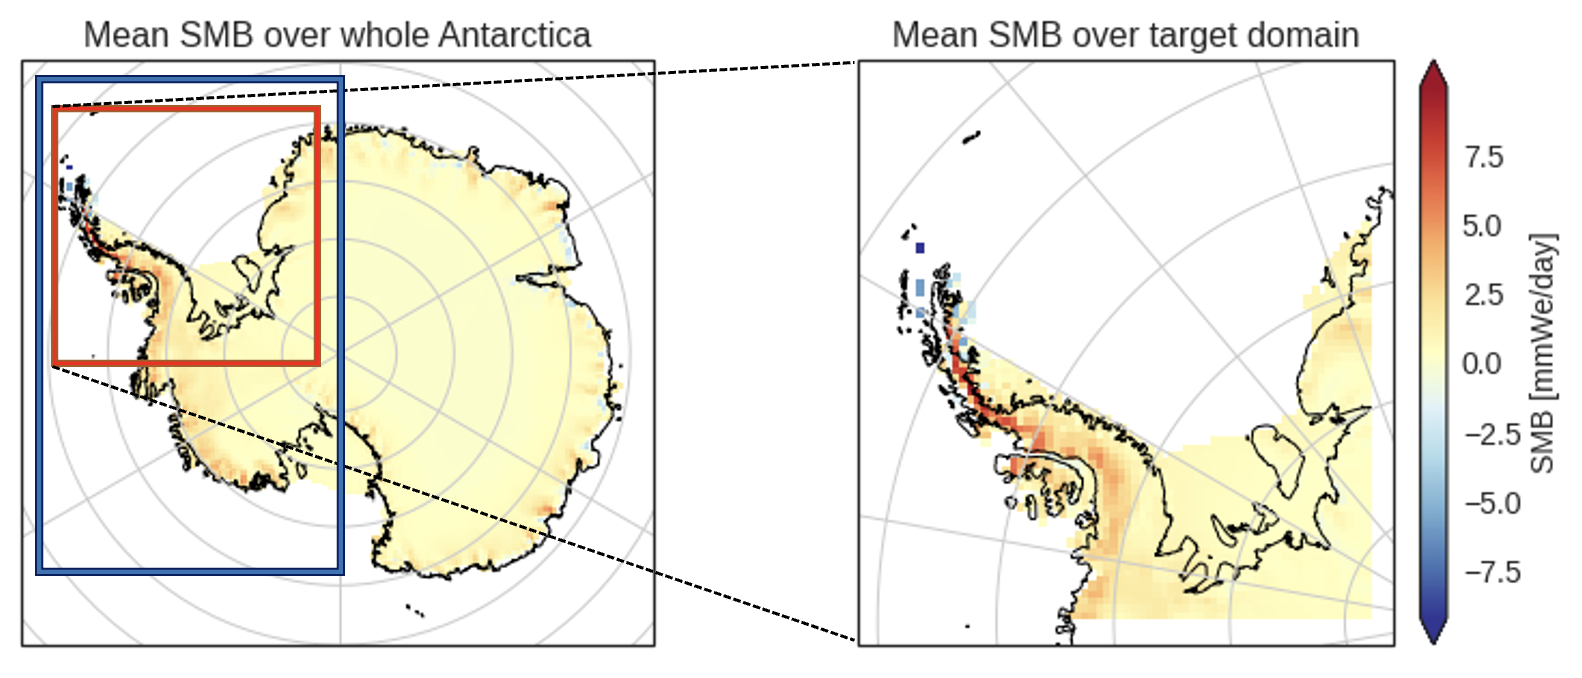
\includegraphics[width=\columnwidth]{images/domains.png}
  \caption []{\small Mean surface mass balance over Antarctica (left) and Antarctic Peninsula (right). Regions chosen as target domain $\mathcal{E}$ (in red) and input domain $\mathcal{D}$ (in blue) for Emulator. }
  \vspace{-3mm}
    \label{fig:region-of-choice}
\end{figure}


\subsection{Target domain}
\begin{itemize}
    \item The target domain used for this model is a grid box of 64x64 at 35km resolution that contains the Antarctic Peninsula in West Antarctica. 
    \item Chosen because Antarctic Peninsula has high annual variability in SMB values, shows high extremes of SMB and SMB values vary greatly across geographical location (Fig.~\ref{fig:region-of-choice})
    \item It covers 5,017,600 square kilometres and is majoritarely covered by ice. Major ice shelves include the Larsen and Ronne ice shelves. 
    \item Peninsula is very mountainous, its highest peaks rising to about 2,800 m
    \item Temperature: because the Antarctic Peninsula, which reaches north of the Antarctic Circle, is the most northerly part of Antarctica, it has the mildest climates within this continent. Its temperatures are warmest in January, averaging 1 to 2$\degree C$, and coldest in June, averages from -15 to -20$\degree C$
    \item Precipitation: varies greatly within the Antarctic Peninsula. The tip of peninsula has highest levels of precipitation with 35–50cm per year. A good portion of this precipitation falls as rain during the summer. On the west coast and along its northeast coast, precipitation is 35cm or less with occasional rain. Along the east coast and the interior of Antarctica, climate is drier with precipitation that ranges from 10-15 cm~\cite{antarctic-climate, antarctic-climate-2}.
    \item This shows when looking at mean SMB values. The tip of the peninsula and its west coast show higher values than the rest (Fig.~\ref{fig:region-of-choice}). Mean SMB ranges from -9.2 to 9.9 mmWe/day and the extremes observed in this region over the whole time-frame of 1980-2100 are a minimum of -59.0 mmWe/day and a maximum of 30.2 mmWe/day
\end{itemize}

\subsection{Perfect model framework}
\begin{itemize}
    \item The authors of~\cite{Kittel} trained their U-Net emulator in a \textit{perfect model framework} where both inputs and outputs to the model come from the same RCM simulation. They give several reasons for this: 
    \begin{itemize}
        \item the aim of the study is to learn the downscaling function of the RCM
        \item for this, we need perfect consistency (temporal and spatial correlation) between low-resolution inputs and a high-resolution targets. Otherwise, the emulator will try to learn a non-existing or non-exact relationship
        \item this is not guaranteed between GCM and RCM because of large scale biases and inconsistencies. 
    \end{itemize}
    \item We follow the same reasoning, because of this, we create GCM-like features ($\operatorname{UPRCM}$) by upscaling RCM simulation outputs to GCM resolution (about 68x206km) with conservative interpolation (Fig.~\ref{fig:training-data-flow}). 
    \item In a second step, these UPRCM outputs are smoothed by a 3x3 moving average filter. This allows the grid of the GCM to be conserved, but each point contains now smoother information and this further ensures to delete local scale information which might persist through the upscaling~\cite{Doury, Klaver2020}. (The authors of~\cite{Doury, Klaver2020} argue that the effective resolution of climate models is often larger (about 3 times) than its nominal resolution and that for this reason a GCM cannot be trusted at its own horizontal resolution but only at a coarser resolution.)
\end{itemize}
\subsection{Input features}
\begin{itemize}
    \item The features $(X, Z)$ provided as input to the emulator consist of two-dimensional variable $X$, and one-dimensional $Z$ (Table~\ref{tab:features}). 
    \item The two-dimensional feature $X$ contains eight different atmospheric variables measured at surface level. \item These eight variables were present both in our RCM and GCM data. In terms of feature selection, we decided to follow the same procedure as in~\cite{Doury} and give all available variables to the model and let it find the right combination to be used [COMPLETE WITH FEATURE SELECTION RESULTS]. 
    \item These variables are z-score normalised according to their monthly spatial mean $\bar{X}_{t,x}$ and standard deviation $\sigma(X_{t,x})$:
    \begin{equation}\label{eq:normalisation-X}
    \tilde{X}_{t,i,j,x} = \frac{X_{t,i,j,x}-\bar{X}_{t,x}}{\sigma(X_{t,x})} \;\;\;\; t\in T, \forall (i,j) \in \mathcal{D}, x\in C_2
\end{equation}

\item The one-dimensional variable $Z$ includes the monthly spatial means $\bar{X}_{t,x}$ and standard deviations $\sigma(X_{t,x})$ time-series for each 2D variable because the 2D variables are normalised at each time step by their spatial mean and so don’t carry any temporal information
\item It also includes a cosinus, sinus vector to encode the information about the month of the year.
\begin{equation}
    \operatorname{cos}\left(\frac{2\pi t}{12}\right);\; \operatorname{sin}\left(\frac{2\pi t}{12}\right) \;\;\;\; t\in T
\end{equation}
\item As in~\cite{Doury}, in order to always give normalised inputs to the emulator, the spatial means $\bar{X}_{t,x}$ and standard deviations $\sigma(X_{t,x})$ in Z are normalised according to the means and standard deviations of $\bar{X}_{ref,x}$ and $\sigma(X_{ref,x})$ over a reference period ($ref=$1980-2000).
\begin{equation}\label{eq:normalisation-Z}
    \tilde{Z}_{t,z} = \frac{Z_{t,z}-\bar{Z}_{ref,z}}{\sigma(Z_{ref,z})} \;\;\;\; t\in T, z\in C_1
\end{equation}
where $\bar{Z}_{ref,z}$ and $\sigma(Z_{ref,z})$ are respectively the temporal mean and standard deviation of the spatial means or standard deviation of $X_{ref, x}$.
 \item Input domain: $48\times25$ grid box (Fig.~\ref{fig:region-of-choice}) defined around the target domain (Antarctic Peninsula) that is resized to $32\times 32$ by bilinear interpolation so as to give the model a square input.
\item Input to model: Each observation given to the emulator is a month $t$ and is an array $X \in I \times J \times C_1$, where the two first dimensions are the spatial coordinates and the number of channels $C_1$ are the different atmospheric variables chosen as predictors, and its corresponding one dimensional $Z \in C_2$ (Fig.~\ref{fig:example-features}).
\end{itemize}

\begin{table}[tbp]
    \centering
    \caption{}
    \renewcommand\arraystretch{1.5}
    \begin{tabular}{l>{\centering}p{0.1\linewidth}>{\centering}p{0.2\linewidth}>{\centering\arraybackslash}p{0.2\linewidth}}
    \toprule
        \textbf{Variable Name} & \textbf{Variable Notation} & \textbf{Units} & \textbf{Dimensions} \\ \toprule
        \textbf{2D variables} & & & \\ \bottomrule 
        Northward Wind & NW & $[ms^-1]$ & $ \mathcal{D}$   \\ 
        Eastward Wind & EW & $[ms^-1]$ & $ \mathcal{D}$ \\
        Downwelling Shortwave Radiation & SWD & $[Wm^{-2}]$ & $ \mathcal{D}$ \\
        Downwelling Longwave Radiation & LWD & $[Wm^{-2}]$ & $ \mathcal{D}$ \\
        Specific Humidity & QQP & $[g/Kg]$ & $ \mathcal{D}$ \\
        Temperature & TT & $[\degree]$ & $ \mathcal{D}$ \\
        Precipitation & PR & $[mmWe/day]$ & $ \mathcal{D}$  \\
        Pressure & PR & $[hPa]$ & $ \mathcal{D}$  \\
        \toprule
         \textbf{1D variables} & & & \\ \bottomrule
        Spatial mean of 2D variables & $\bar{X}_{x}$ & & $[C_1]$ \\ 
        Spatial std of 2D variables & $\sigma\left(X_{x}\right)$ & & $[C_2]$ \\
        Seasonal Indicators & & & $[2]$\\ \bottomrule
        
    \end{tabular}
        \subcaption*{\small Table~\ref{tab:features}. Two and one-dimensional input features given to the model. Each feature is measured (near) surface and a monthly mean aggregation.}
            \label{tab:features}
\end{table}


\begin{figure}[!t]
  \centering
  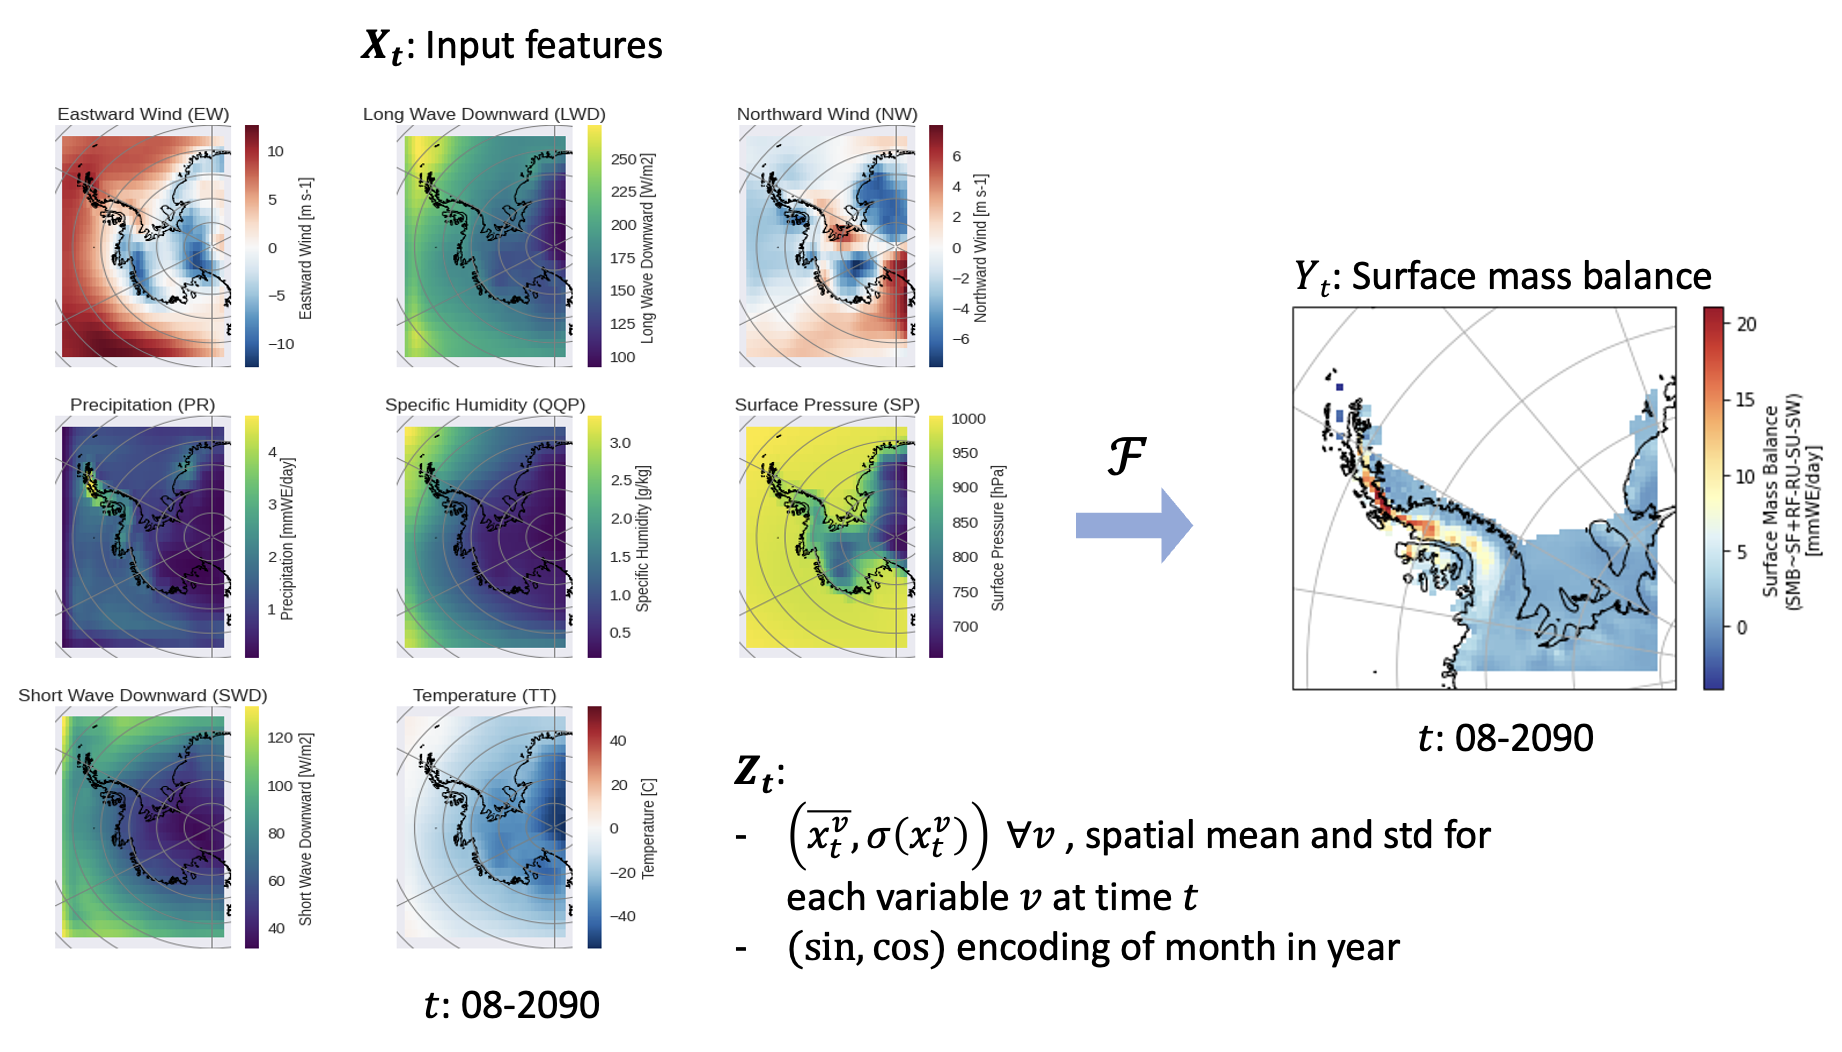
\includegraphics[width=\columnwidth]{images/data_example.png}
  \caption []{\small Illustration of an observation at time-step $t$. Left: 2D input variables $X_t$ on the input domain with its corresponding 1D variable $Z_t$. before they're normalised. Right: the target surface mass balance (SMB) $Y_t$ on the target domain.}
  \vspace{-3mm}
  \label{fig:example-features}
\end{figure}






\section{Architecture}\label{sec:model}
\begin{itemize}
    \item Our architecture is an extension of the SmaAt-UNet model proposed in~\cite{smatunet}.
     \item SmaAt-UNet extends the traditional U-Net architecture~\cite{unet} with CBAM attention mechanism and depthwise-separable convolutions instead of regular convolutional operations. 
    \item Traditional U-Net is a fully convolutional CNN architecture specifically developed for biomedical image segmentation~\cite{Ronneberger2015}. 
    \item U-Net shows high performance in classification and segmentation tasks where the network is trained to predict a class for each pixel. But U-Nets are also used for image processing tasks, such as super resolution. They have been found to be particularly effective in cases where the output and inputs are of similar size. In our case, we applied it to a time series prediction task in which the network has to predict an exact value for each pixel.

    \item The network is U-shaped as it is divided into a down-sampling/encoder section that forms the left side and an up-sampling/decoder for the right.
    \item Encoder: max-pooling (red arrows) and a double convolution (blue arrows) which halves the image size and doubles the number of channels
    \item Decoder: three parts: a 2D transposed convolution operation (green arrows) to double the feature map size, a concatenation of the resulting feature maps with the previous encoder’s output via skip-connections (grey arrows), and lastly a double convolution to half the number of feature maps
    \item  Skip-connections between layers make it possible to skip large sections if required and create a smoother loss surface. 
    \item  Last layers: up-sampling layer in order to reach target size and 1 × 1 convolution (purple arrow) which outputs a single feature map representing the SMB values predicted by the network at time-step $t$
    \item Bottom: add a 1-dimensional input $Z$ at bottom of the “U” after a short fully dense network of 4 layers → concatenates encoded spatial information (from $X$) and encoded temporal information (from $Z$). Forces U-net to give the same importance to 2 inputs before starting decoding path and recreating the high resolution SMB map. 
    \item CBAMs: using attention in a CNN facilitates the network to focus on specific parts of the input. For our model, we use convolutional block attention modules for the purpose of identifying important features across channels and spatial regions of the image. In CBAMs, the attention mechanism is applied first across the channels of the image and subsequently to the spatial dimension. The CBAMs are placed after the first double convolution and every encoder to amplify important features and suppress unimportant ones on the respective image scale (yellow arrows in Fig.~\ref{fig:UNet-architecture}). Importantly, the input to the encoders is the convoluted and downsampled image from the previous encoder and not the image with the attention mechanism applied. This way, the original image features are preserved until the last encoder. The attention modules only feed into the corresponding upsampling part of the network to which they are connected through the skip-connections.
    \item DSC: instead of usual double convolutions, use depthwise-separable convolutions to reduce the number of parameters. In particular, replace all convolutions of the original U-Net model with depthwise-separable convolutions. However, in the convolutional block attention modules we still apply regular convolutions. 
    \item Architecture implemented in PyTorch 1.11
\end{itemize}

\begin{figure}[!t]
  \centering
  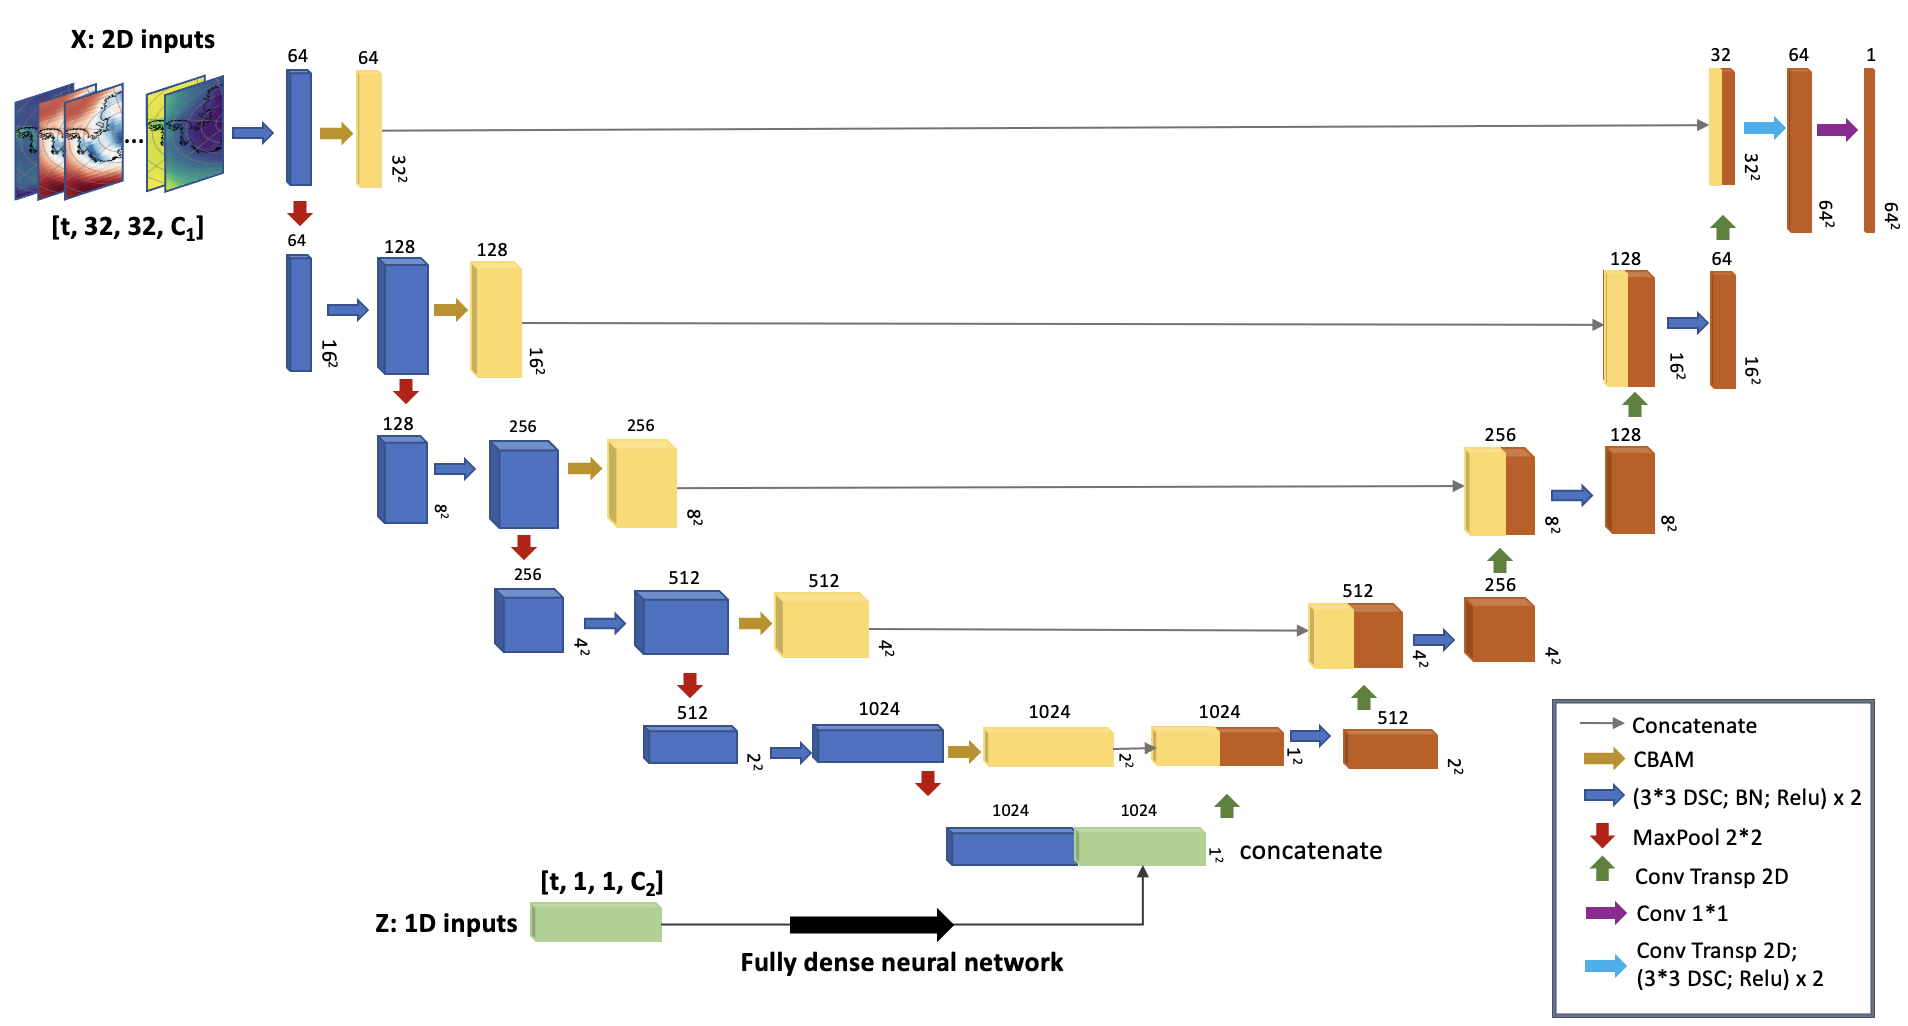
\includegraphics[width=\columnwidth]{images/smatunet.png}
  \caption []{\small Scheme of the neural network architecture used for this paper. The part of the network in the red frame corresponds to the original U-Net defined in \cite{unet}. Image reproduced from~\cite{Doury}.}
  \vspace{-3mm}
  \label{fig:UNet-architecture}
\end{figure}

\section{Training}\label{subsec:training}
\subsection{Perfect model framework}\label{subsec:perfect-model-training}
\begin{figure}[!t]
  \centering
  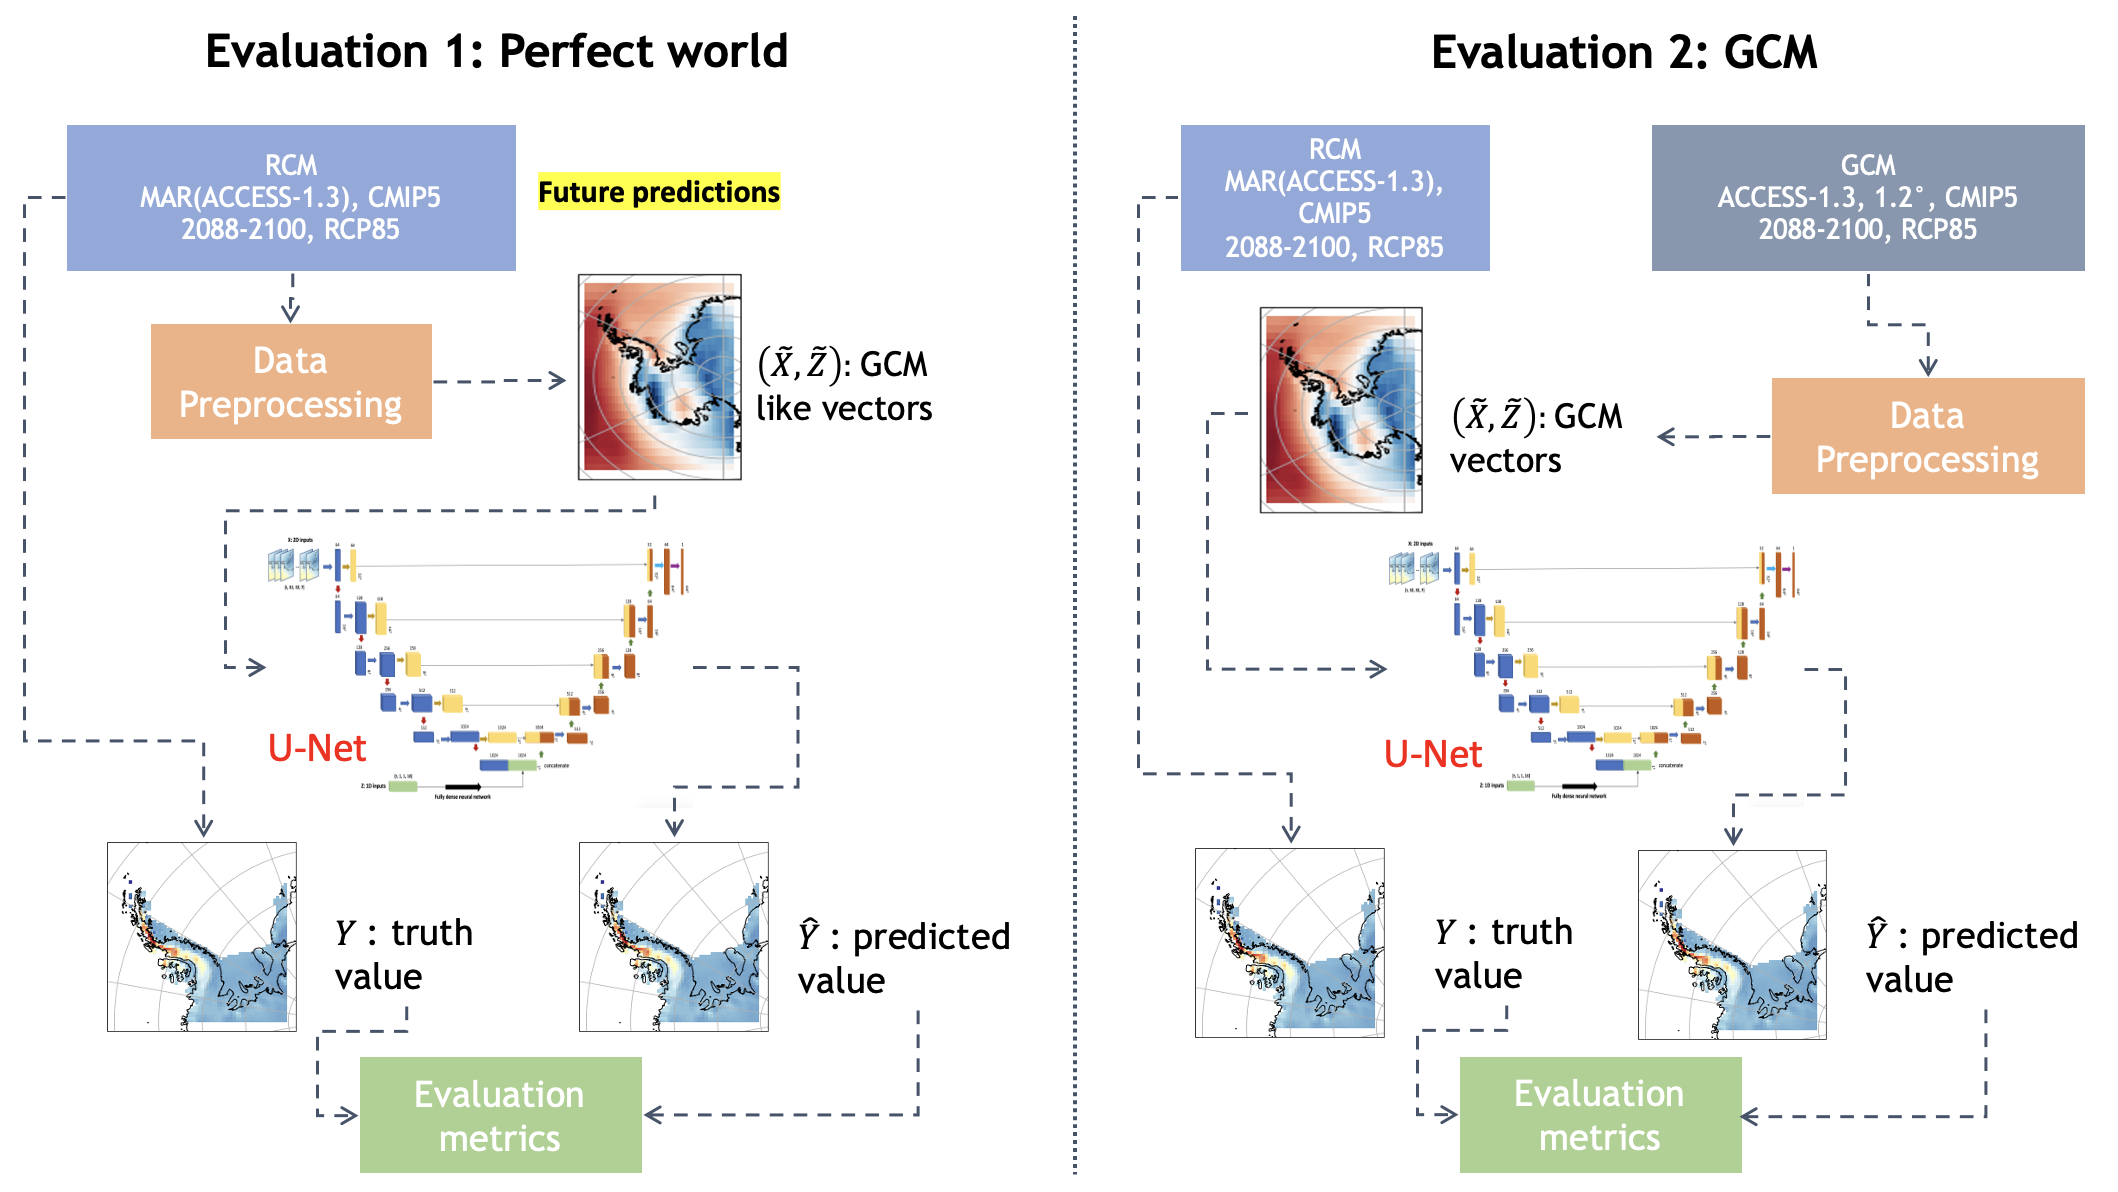
\includegraphics[width=\columnwidth]{images/evaluation-framework.png}
  \caption []{\small Evaluation framework}
  \vspace{-3mm}
  \label{fig:UNet-architecture}
\end{figure}


\subsection{Loss}\label{subsec:loss}
As a loss, we use the same as the authors of~\cite{Doury} that propose to view the problem as a regression and used Mean Squared Error (MSE). At each pixel location $p$ in domain $\mathcal{D}$, the MSE measures the average squared difference between the predicted values $\widehat{Y_{p}}$ and the ground truth $Y_{p}$:
\begin{equation}
        \operatorname{MSE}\left(Y_{p},\widehat{Y_{p}}\right) = \frac{1}{T}\sum_{t}(\hat{y}_{p}^{t}-y^{t}_{p})^2   \;\;\;\; \forall p \in \mathcal{D} 
\end{equation}
where $\hat{y}_{p}^{t}$ is the SMB value predicted at location $p\in \mathcal{D} $ and time step $t$.

\subsection{Early stopping}
\subsection{LR scheduler}


\section{Evaluation}\label{sec:evaluation}

\subsection{Framework}\label{subsec:evaluation-framework}
As previously mentioned in~\ref{subsec:perfect-model-training}, the model is trained in a perfect model framework, where both its low resolution inputs and high resolution output come from the same regional climate model.
\begin{itemize}
\item If RCP 4.5 not available, train model on 90\% of time series i.e. from 1980 till 2080 and evaluate on future scenario 2080-2100. 
    \item If RCP 4.5. avaible, train on RCP 8.5 and evaluate on whole time series of RCP 4.5.
    \item In a second evaluation step, evaluate with inputs from GCM 
\end{itemize}


\subsection{Evaluation metrics}\label{subsec:evaluation-metrics}
At each position $p$ in domain $\mathcal{D} $ of the regional climate model grid, the truth series ($Y_{p}$) from the regional climate model are compared the predicted values $\widehat{Y_{p}}= \theta(Y_{pp})$ by the emulator $\theta$. For this, we use the same statistical scores the authors of~\cite{Doury} used to evaluate their downscaling model. Each of these metrics is computed over the complete period from $t_{0}=31.01.1980$ to $t_{N}=31.12.2100$:
\subsubsection{RMSE}\label{subsubsec:rmse}
The Root Mean Squared Error (RMSE) is a measure of the difference between predictions of an estimator and the observed values. RMSE is the square root of the average of squared differences between prediction and actual observation. It is also defined as the square of the Mean Squared Error (MSE):
\begin{align}
        \operatorname{RMSE}\left(Y_{p},\widehat{Y_{p}}\right) & = \sqrt{\operatorname{MSE}\left(Y_{p},\widehat{Y_{p}}\right)} \\ & = \sqrt{\frac{1}{T}\sum_{t}(\hat{y}_{p}^{t}-y^{t}_{p})^2} & \forall p \in \mathcal{D} 
\end{align}
where $\hat{y}_{p}^{t}$ is predicted SMB value and $y^{t}_{p}$ the true SMB value at location $p\in \mathcal{D} $ and time step $t$. The amplitudes of SMB time series varies according to geographical location i.e., some locations that are very dry may have SMB values that vary between 0 and 1 mmWe/day while others may go up to 10 mmWe/day. For this reason, we also compute the normalised RMSE (NRMSE):
\begin{align}
        \operatorname{NRMSE}\left(Y_{p},\widehat{Y_{p}}\right) & = \frac{\operatorname{RMSE}\left(Y_{p},\widehat{Y_{p}}\right)}{Y_{max}(p) - Y_{min}(p)} \\ & = \frac{\frac{1}{T}\sum_{t}(\hat{y}_{p}^{t}-y^{t}_{p})^2}{Y_{max} - Y_{min}} & \forall p \in \mathcal{D} 
\end{align}
where $Y_{max}$ and $Y_{min}$ are respectively the maximum and minimum true SMB values over the whole domain $\mathcal{D}$. 


\subsubsection{Pearson correlation}\label{subsubsec:pearson}
Pearson correlation coefficient measures how two continuous signals co-vary over time and indicate the linear relationship as a number between -1 (negatively correlated) to 0 (not correlated) to 1 (perfectly correlated).
\begin{align}
    \rho\left(Y_{p},\widehat{Y_{p}}\right) = \frac{\operatorname{cov}(Y_{p},\widehat{Y_{p}})}{\sigma_{Y_{p}}\sigma_{\widehat{Y_{p}}}} \;\;\;\; \forall p \in (x,y)
\end{align}
where $\operatorname {cov}$  is the covariance and  $\sigma$ is the standard deviation.

\subsubsection{Wasserstein distance}\label{subsubsec:wasserstein}
The Wasserstein distance is the numerical cost of an optimal transportation problem i.e., the cost of
the optimal transport plan~\cite{villani} for moving the mass in the predicted
measure to match that in the target~\cite{wasserstein1}. It measures the distance between two probability density functions $f(\cdotp)$, in our case $f(Y_p)$ and $f(\widehat{Y_p})$.
\begin{equation}
    \operatorname{W}\left(f(Y_p),f(\widehat{Y_p})\right) = \sum_{t}|y^{t}_{p}-\hat{y}_{p}^{t}| \;\;\;\; \forall p \in (x,y)
\end{equation}
 where $\hat{y}_{p}^{t}$ is the SMB value predicted at location $p\in (x,y)$ and time step $t$.

\subsubsection{Variance ratio}\label{subsubsec:variance-ratio}
 The variance ratio measures the performance of the emulator in reproducing local monthly variability. 
 \begin{equation}
     \operatorname{F}(Y_{p},\widehat{Y_{p}}) = \frac{\operatorname{Var}(\widehat{Y_{p}})}{\operatorname{Var}(Y_{p})}\cdot100
 \end{equation}
 where $\operatorname{Var}(Y)$ is the variance $\sigma^2$ of sample $Y$. The authors of~\cite{Doury} express this measure as a percentage. 



%%%%%%%%%%%%%%%%%%%%
\chapter{Results}
%%%%%%%%%%%%%%%%%%%%

In the evaluation you convince the reader that your design works as intended.
Describe the evaluation setup, the designed experiments, and how the
experiments showcase the individual points you want to prove.

This section is usually 5-10 pages.

\section{Results on RCM}
\subsection{Some time-series}

% Histogram distances
\begin{figure}[tbp]
        \centering
        \begin{subfigure}[b]{0.8\columnwidth}
            \centering 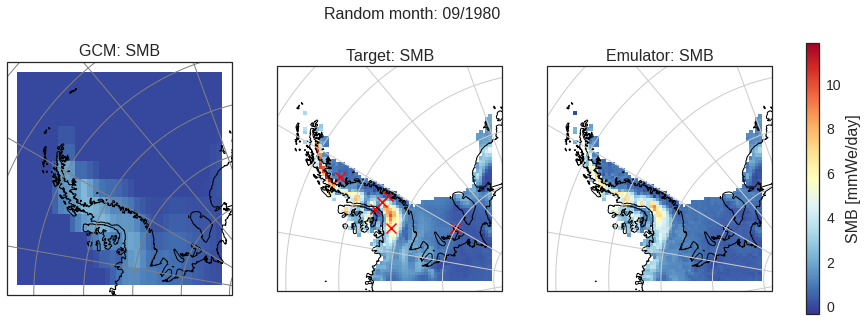
\includegraphics[width=\textwidth]{images/random_month_RCM.png}
            \caption[]%
            {{\small Random month 09/1980}}    
          \label{fig:rdpoints-RCM}
        \end{subfigure}
        \hfill
        \begin{subfigure}[b]{\columnwidth}  
            \centering 
            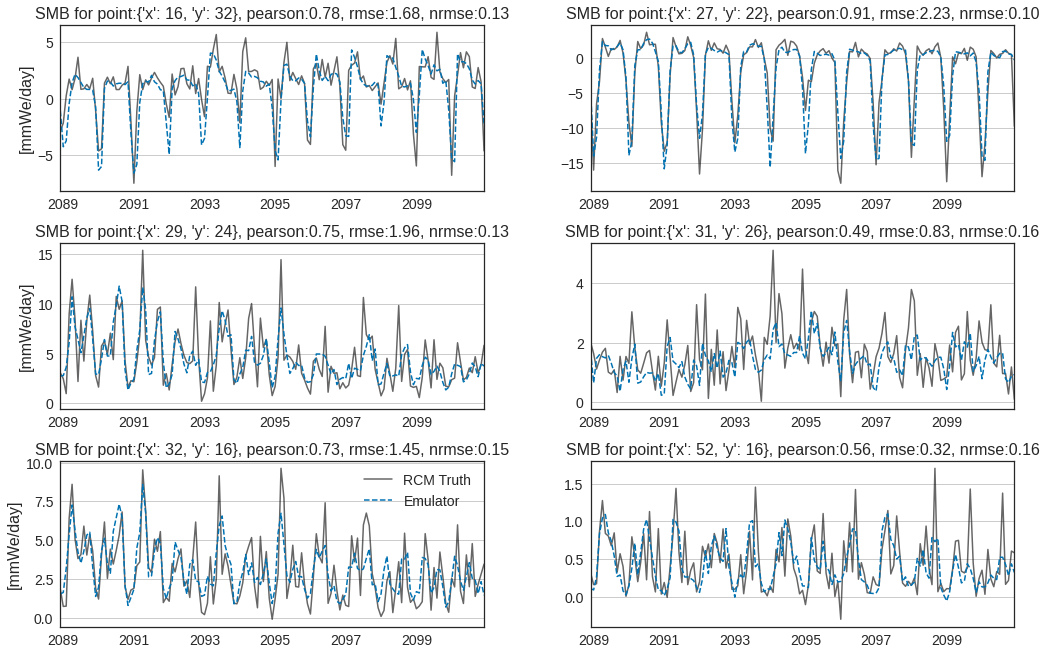
\includegraphics[width=\textwidth]{images/timeseries_RCM.png}
            \caption[]%
            {{\small Time series}}  
            \label{fig:timeseries-RCM}
        \end{subfigure}
        \hfill
        \caption[]
        {\small Randomly chosen illustration of the production of the emulator: (a) SMB at a random month over the target domain $\mathcal{E}$ for the GCM, RCM truth and emulator, and (b) random future time series for 6 particular grid points.} 
        \label{fig:points-timeseries-RCM}
    \end{figure}


\subsection{Evaluation metrics}


\section{Results on GCM}

%%%%%%%%%%%%%%%%%%%%
\chapter{Discussion}
%%%%%%%%%%%%%%%%%%%%

In the evaluation you convince the reader that your design works as intended.
Describe the evaluation setup, the designed experiments, and how the
experiments showcase the individual points you want to prove.

This section is usually 5-10 pages.



%%%%%%%%%%%%%%%%%%%%
\chapter{Conclusion}
%%%%%%%%%%%%%%%%%%%%

In the conclusion you repeat the main result and finalize the discussion of
your project. Mention the core results and why as well as how your system
advances the status quo.

\cleardoublepage
\phantomsection
\addcontentsline{toc}{chapter}{Bibliography}
\printbibliography

% Appendices are optional
\appendix
% %%%%%%%%%%%%%%%%%%%%%%%%%%%%%%%%%%%%%%
\chapter{Data processing}
\begin{figure}[!t]
  \centering
  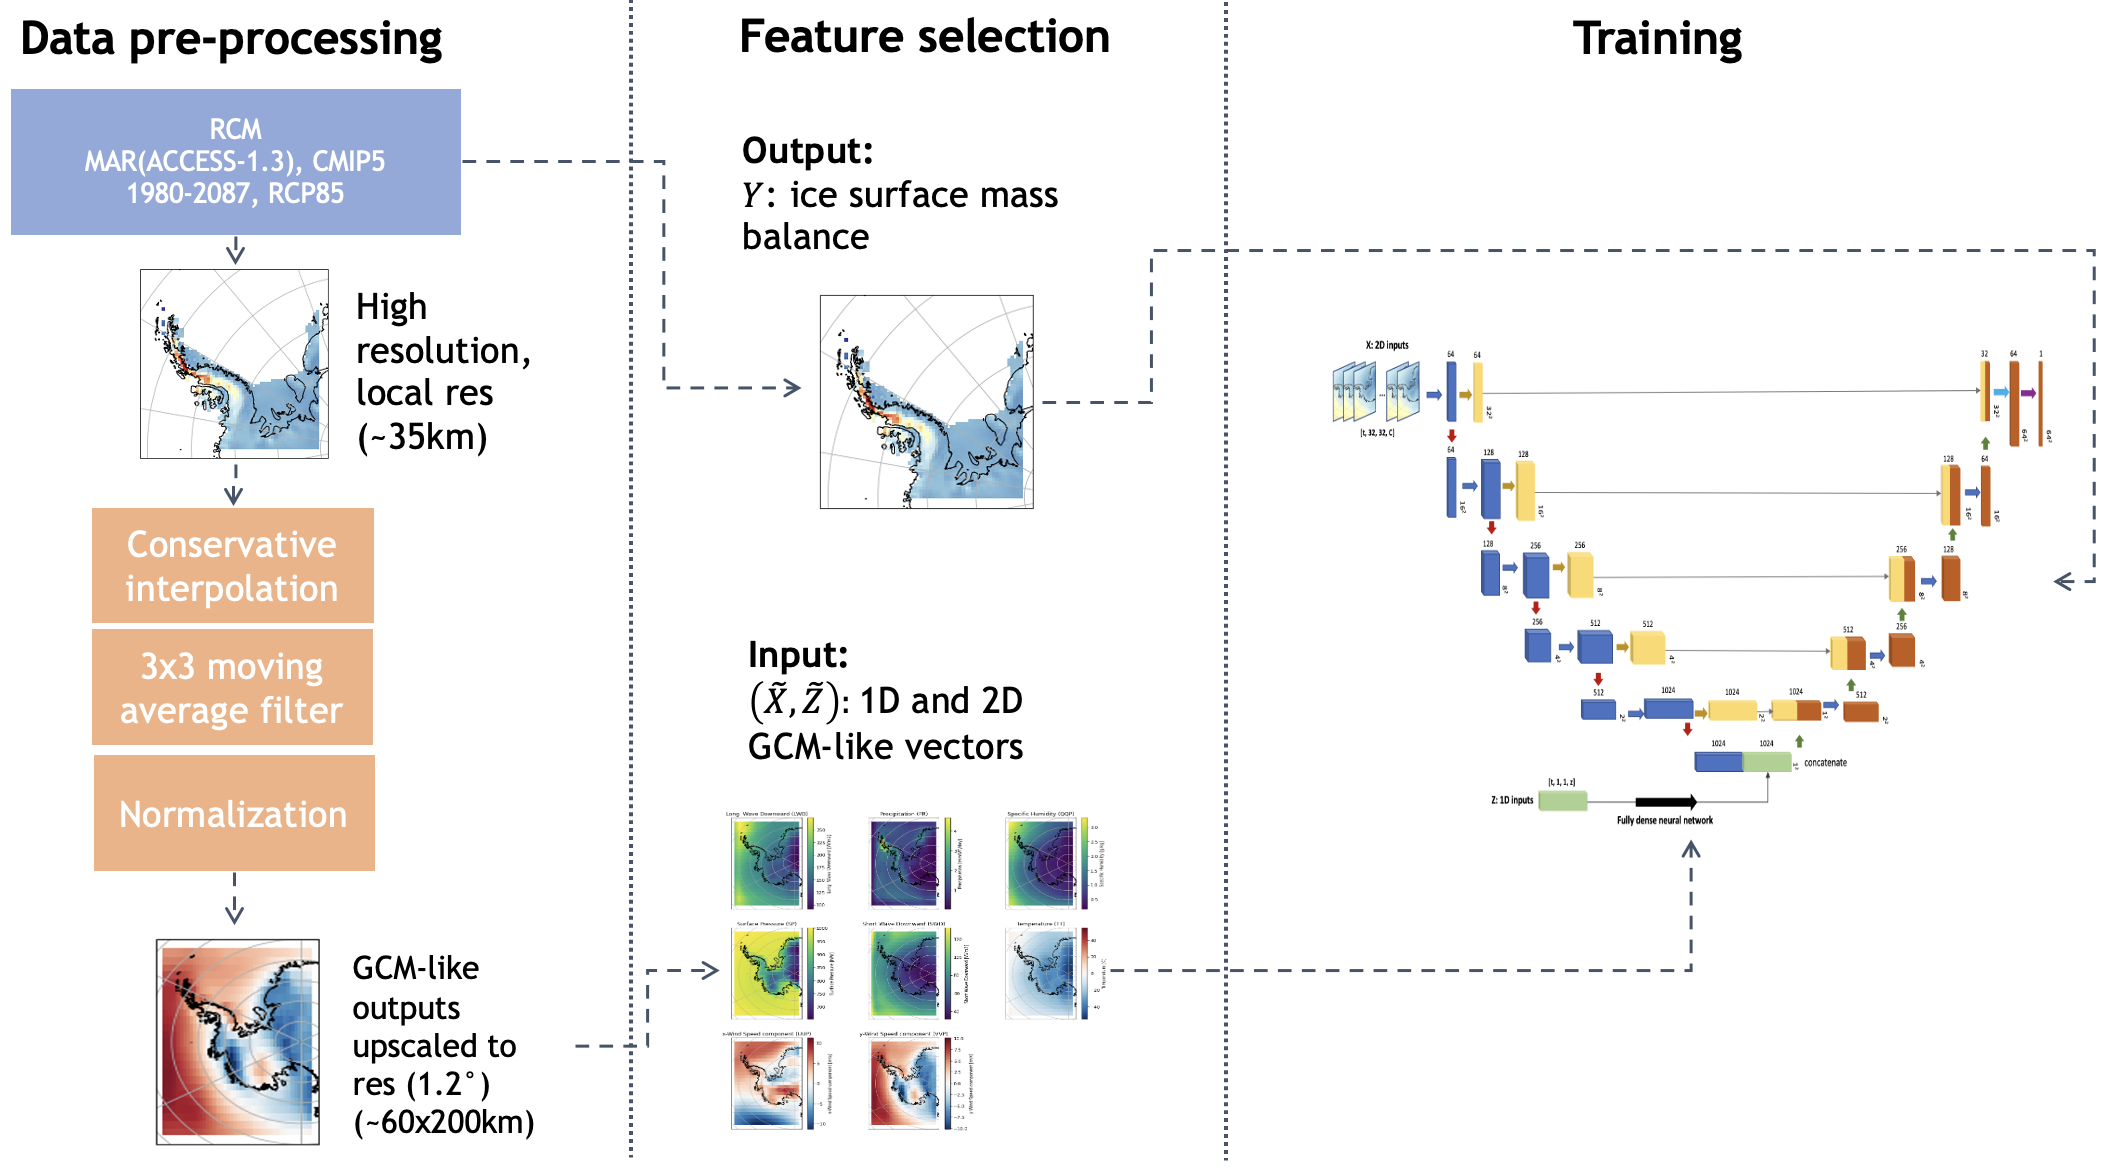
\includegraphics[width=\columnwidth]{images/data-flow.png}
  \caption []{\small Training data flow}
  \vspace{-3mm}
  \label{fig:training-data-flow}
\end{figure}
\section{Pre-processing of RCM}
\begin{itemize}
    \item  Because GCM data we have is monthly frequency, do monthly mean aggregation for RCM data.

\end{itemize}
\section{Pre-processing of GCM}
\chapter{Feature selection}
\section{Feature selection RCM}
\section{Feature selection GCM}

\chapter{Hyperparameter tuning}
% %%%%%%%%%%%%%%%%%%%%%%%%%%%%%%%%%%%%%%

\begin{table}[tbp]
    \centering
    \caption{}
    \renewcommand\arraystretch{1.5}
    \begin{tabular}{l>{\centering}p{0.1\linewidth}>{\centering}p{0.1\linewidth}>{\centering}p{0.05\linewidth}>{\centering}p{0.05\linewidth}>{\centering}p{0.05\linewidth}>{\centering}p{0.1\linewidth}>{\centering}p{0.05\linewidth}>{\raggedright\arraybackslash}p{0.05\linewidth}}
    \toprule
        Model & x & y & Batch size & Num epochs & Weight decay & learning rate & Train loss & Val loss \\ \toprule
        Simul 2 & (3, 500, 500) & (3, 500, 500) & 4 & 10 & 1e-3 & 0.01 & 0.5513 & 0.5490 \\ 
        Sim 3 & (3, 250, 250) & (3, 250, 250) & 20 & 10 & 1e-3 & 0.01 & 0.6505 & 0.6240 \\ 
        Sim 4 & (3, 250, 334) & (3, 250, 334) & 15 & 10 & 1e-3 & 0.01 & 0.6056 & 0.5875 \\ 
        Sim 5 & (3, 250, 334) & (3, 250, 334) & 15 & 10 & 1e-3 & 0.01 & 0.6043 & 0.5753 \\ 
        Sim 6 & (3, 250, 334) & (3, 250, 334) & 15 & 10 & 1e-3 & 0.01 & 0.4498 & 0.5015 \\ 
        Sim  7 & (3, 250, 334) & (3, 250, 334) & 15 & 10 & 1e-3 & 0.01 & 0.3511 & 0.3460 \\ 
        Sim  8  & (3, 250, 334) & (3, 250, 334) & 15 & 10 & 1e-3 & 0.01 & 0.6199 & 0.6041 \\ 
        Sim 9 & (3, 250, 334) & (3, 250, 334) & 15 & 10 & 1e-3 & 0.01 & 0.5916 & 0.5254 \\ \bottomrule
    \end{tabular}
        \subcaption*{\small Table~\ref{tab:phase1a}. Phase 1a. \textbf{Validation and training loss}: value at the end of the last epoch. \textbf{x and y}: input and output given to the model during training. }
            \label{tab:phase1a}
\end{table}
% In case you ever need an (optional) appendix.
%
% You need the following items:
% \begin{itemize}
% \item A box
% \item Crayons
% \item A self-aware 5-year old
% \end{itemize}

\end{document}